\documentclass{beamer}
\usepackage[latin1]{inputenc}
\usepackage[brazil]{babel}
\usepackage{graphicx}
\usetheme{JuanLesPins}
\title{\bf Projeto Interativo II \\ Desenvolvimento de jogo 2D}
\author{Davi S. Meneses - davismeneses@hotmail.com \\ Jennifer Cintra P. Silva - jennifer.cintra.03@gmail.com \\ Jesley Silva de Oliveira - dhiesleyolivera@yahoo.com.br \\ Raldney Sampaio Alves - raldney{\_}sampaio@hotmail.com}
\institute{Centro Universit�rio SENAC}
\date{Setembro de 2013}
\begin{document}
\begin{frame}[plain]
\titlepage
\end{frame}
\begin{frame}
\frametitle{Sum�rio}
 - Introdu��o;\\
 - O Jogo;\\
 - Jogabilidade;\\
 - Conclus�o.
\end{frame}
\begin{frame}
\frametitle{Introdu��o}
Para o desenvolvimento de um bom jogo n�o � preciso apenas pensar na jogabilidade temos que pensar em como a pessoa esta envolvida com ele, por isso existe uma grande preocupa��o com a historia e com o desing gr�fico, para fazer com que a intera��o jogador x jogo seja a  maior poss�vel. 
\end{frame}
\begin{frame}
\frametitle{O Jogo}
O Jogo em si relata a vida de uma personagem que n�o se preocupa muito com os estudos.\\
Ela sempre tira notas baixas e briga com seus pais. Sai de uma escola boa e vai estudar em um Internato, depois de conversar com seus pais em rela��o �s notas e o comportamento escolar dela.A ida para um Internato representa uma granda mudan�a e ela est� disposto a mudar de uma forma positiva.
\end{frame}
\begin{frame}
\frametitle{Jogabilidade}
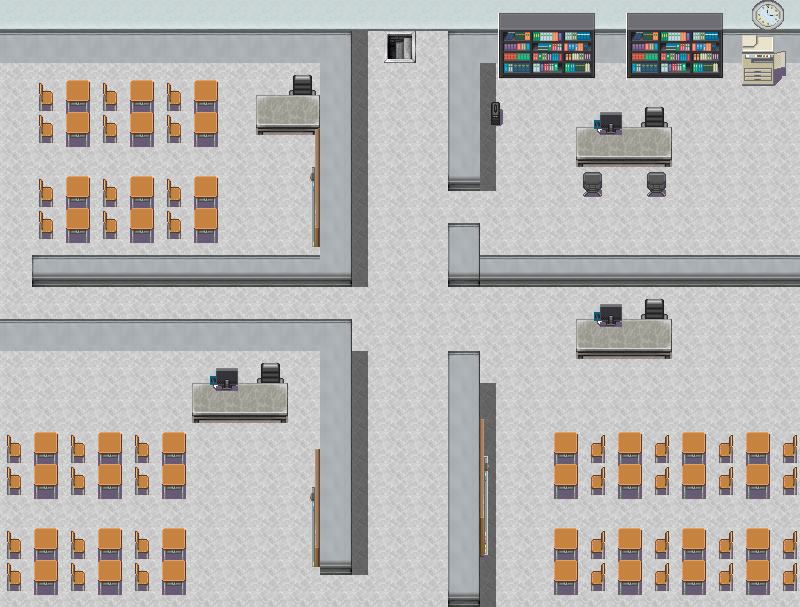
\includegraphics{Salas-Diretor.jpg}
\end{frame}
\begin{frame}
\frametitle{Conclus�o}
A inclus�o de jogos na educa��o de crian�as,jogos pr�prios para eles, podem significar uma grande mudan�a no mundo do aprendizado,se tornando, talvez,uma forma inovadora de ensin�-las o essencial ou o b�sico,assuntos para abordar n�o ir�o faltar e,certamente,alguns outros n�o podem faltar.Ensinar pode ser dif�cil mas,alguns tem ideias que tornam isso simples,pr�tico e funcional.
\end{frame}
\begin{frame}
  \center{\large \bf Agredecemos sua aten��o !}
\end{frame}
\end{document}
